\subsubsection{UC14 - Deploy di funzione}
\begin{figure}[h]
	\centering
	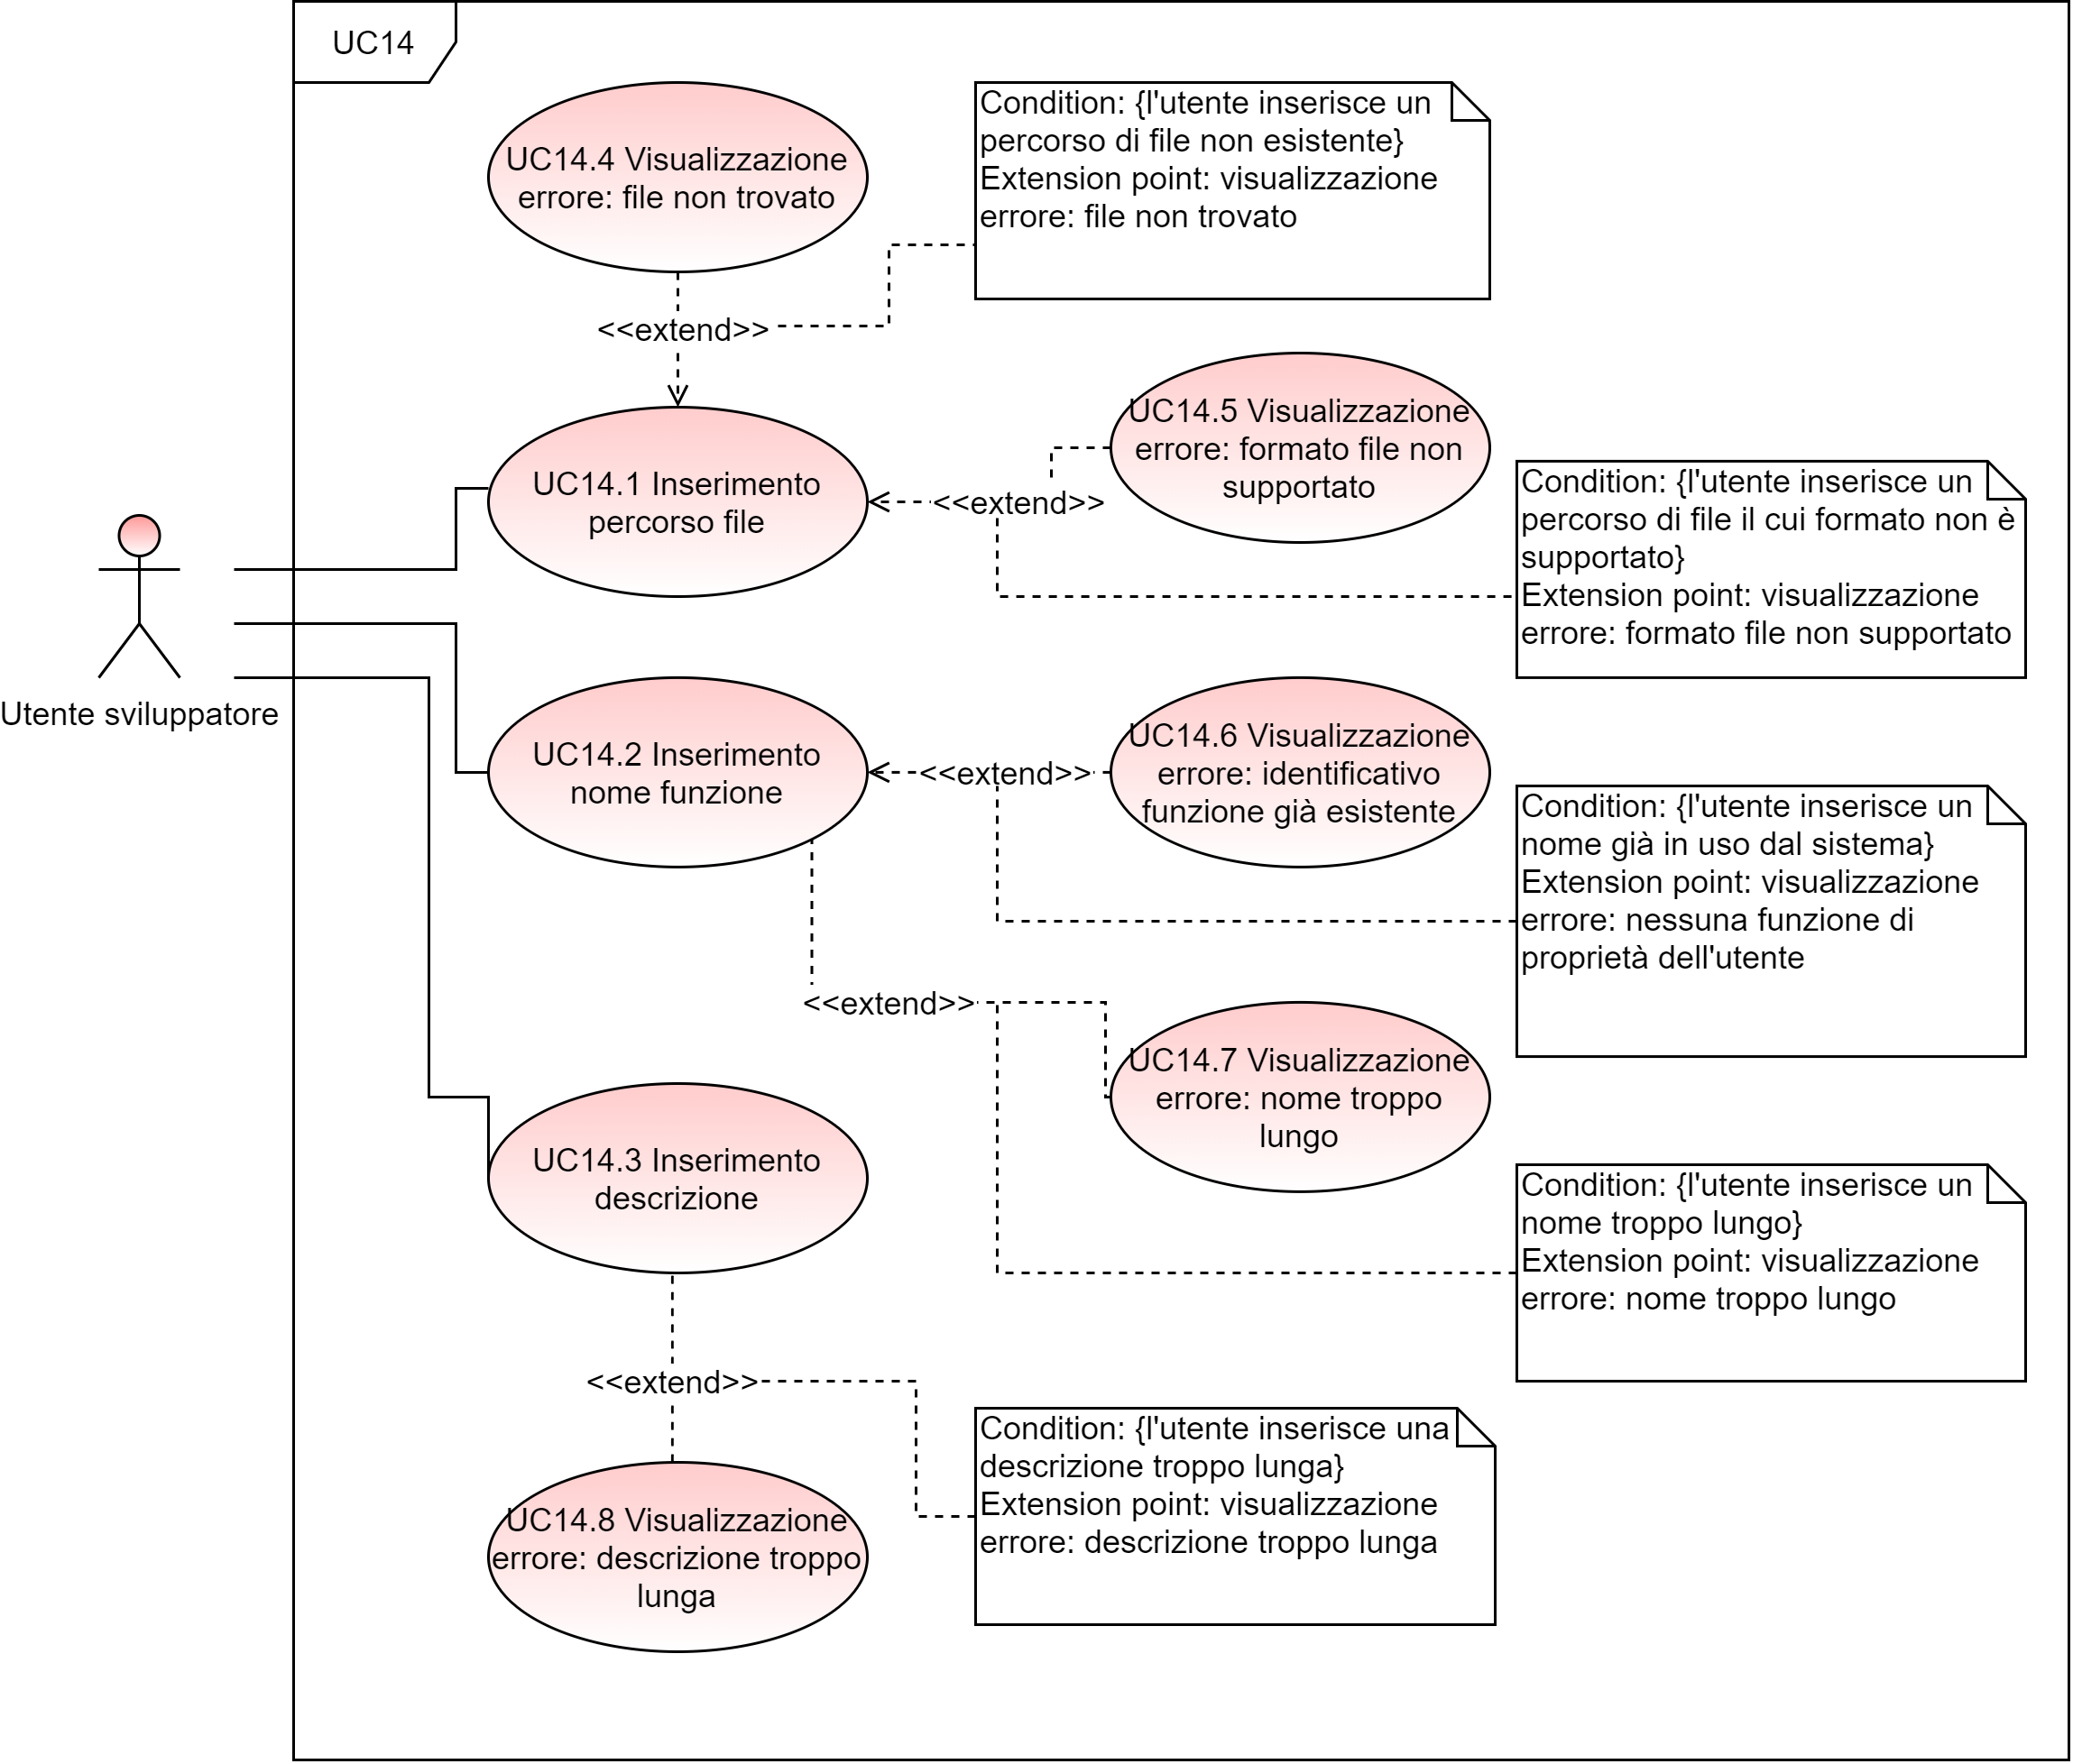
\includegraphics[scale=\ucs]{./res/img/UC14.png}
	\caption {UC14 - Deploy\ped{\textit{G}} di funzione}
\end{figure}
\begin{itemize}
	\item \textbf{Attori primari:} \us{};
	\item \textbf{Attori secondari:} \re{};
	\item \textbf{Descrizione:} l’utente richiede di pubblicare una funzione eseguendo il comando \pdeploy{}. Il sistema pubblica la funzione; 
	\item \textbf{Scenario principale:} 
	\begin{itemize}
		\item l'utente inserisce correttamente ed esegue il comando \pdeploy{};
		\item la funzione viene pubblicata. 
	\end{itemize}
	\item \textbf{Estensioni:} 
	\begin{itemize}
		\item \textbf{UC19:} l’utente non dispone di credito sufficiente per pubblicare la funzione, di conseguenza viene visualizzato un messaggio di errore. 
	\end{itemize}
	\item \textbf{Precondizione:} l’utente ha avviato correttamente l’applicativo e desidera eseguire il deploy\ped{\textit{G}} di una funzione; 
	\item \textbf{Postcondizione:} la nuova funzione inserita è disponibile presso il servizio. 
\end{itemize}